% Created 2024-06-16 Sun 00:13
% Intended LaTeX compiler: pdflatex
ocumentclass[10pt]{article}% =================================BASE====================================%
\documentclass[10pt]{report}
\usepackage[left=2cm,right=2cm,top=2cm,bottom=2cm]{geometry} % Marges
\usepackage[T1]{fontenc} % Nécessaire avec FrenchBabel
\usepackage[utf8]{inputenc} % Important pour symboles Francophones, é,à,etc
\usepackage{csquotes} % Recommandé par PDFLatex lors de la compilation. 


% Calligraphie
%\usepackage{lmodern} % Ça, ça set latin modern
%\usepackage{mathrsfs} %Permet la command \mathscr (Lettres attachées genre) \mathscr(B)

% Calligraphie
%\usepackage{pxfonts} % Met le texte ET les maths en Palatino + donne accès à des symboles math
\usepackage{palatino} % Cette commande met seulement le texte en police palatino
\usepackage{lmodern} % Pour les maths?
% Use lmodern for sans-serif
\usepackage{mathrsfs} % Permet la command \mathscr (Lettres attachées genre) \mathscr(B)





% Bibliographie
%\usepackage[backend=bibtex,style=phys,sorting=ynt]{biblatex}
\usepackage[backend=biber,sorting=ynt,style=ieee]{biblatex}
\addbibresource{/home/charlesedouard/Desktop/Travail/Documentation/master-bibliography.bib}



\usepackage{amsmath, amssymb, amsthm} % Symb. math. (Mathmode+Textmode) + Beaux théorèmes.
\usepackage{mathtools,cancel,xfrac} % Utilisation de boîtes \boxed{} + \cancelto{}{}, xfrac
\usepackage{graphicx, wrapfig} % Géstion des figures.
\usepackage{hyperref} % Permettre l'utilisation d'hyperliens.
\usepackage{color} % Permettre l'utilisation des couleurs.
\usepackage{colortbl} % Color tables
\usepackage[dvipsnames]{xcolor} % Couleurs avancées.
\usepackage{titling} % Donne accès à \theauthor, \thetitle, \thedate

% Physique
\usepackage{physics} % Meilleur package pour physicien. 


% Style
\usepackage{lipsum} % For fun
\usepackage{tikz} % Realisation de figures TIKZ.
\usepackage{empheq} % Boite autour de MULTIPLE équations
\usepackage{bbding}

% Français
\usepackage[french]{babel} % Environnements en Français.
% ==============================BASE-(END)=================================%



% ================================SETTINGS=================================%
% Pas d'indentation en début de paragraphe :
\setlength\parindent{0pt}
\setlength{\parskip}{0.15cm}

% Tableaux/tabular
% Espace vertical dans les tabular/tableaux
\renewcommand{\arraystretch}{1.2}
% Couleur des tableaux/tabular
\rowcolors{2}{violet!5}{}

% Couleurs de hyperliens :
\definecolor{mypink}{RGB}{147, 0, 255}
\hypersetup{colorlinks, 
             filecolor=mypink,
             urlcolor=mypink, 
             citecolor=mypink, 
             linkcolor=mypink, 
             anchorcolor=mypink}


\usepackage{titling} % Donne accès à \theauthor, \thetitle, \thedate

% Physique
\usepackage{physics} % Meilleur package pour physicien. 


% Style
\usepackage{lipsum} % For fun
\usepackage{tikz} % Realisation de figures TIKZ.
\usepackage{empheq} % Boite autour de MULTIPLE équations

% Français
\usepackage[french]{babel} % Environnements en Français.
% ==============================BASE-(END)=================================%





% ================================SETTINGS=================================%
% Pas d'indentation en début de paragraphe :
\setlength\parindent{0pt}
\setlength{\parskip}{0.15cm}

% Tableaux/tabular
% Espace vertical dans les tabular/tableaux
\renewcommand{\arraystretch}{1.2}
% Couleur des tableaux/tabular
\rowcolors{2}{violet!5}{}

% Couleurs de hyperliens :
\definecolor{mypink}{RGB}{147, 0, 255}
\hypersetup{colorlinks, 
             filecolor=mypink,
             urlcolor=mypink, 
             citecolor=mypink, 
             linkcolor=mypink, 
             anchorcolor=mypink}


% Numéros d'équations suivent les sections :
\numberwithin{equation}{section} 

% Les « captions » sont en italique et largeur limitée
\usepackage[textfont = it]{caption} 
\captionsetup[wrapfigure]{margin=0.5cm}

% Retirer l'écriture en gras dans la table des matières
\usepackage{tocloft}
\renewcommand{\cftsecfont}{\normalfont}
\renewcommand{\cftsecpagefont}{\normalfont}

% Change bullet style
\usepackage{pifont}
\usepackage{enumitem}
%\setlist[itemize,1]{label=\ding{224}}
\setlist[itemize,1]{label=\ding{239}}
\renewcommand{\boxtimes}{\blacksquare}
% ================================SETTINGS=================================%



% ==============================NEWCOMMANDS================================%

% Vecteurs de base :
\newcommand{\nvf}{\vb{\hat{n}}}
\newcommand{\ivf}{\vb{\hat{i}}}
\newcommand{\jvf}{\vb{\hat{j}}}
\newcommand{\kvf}{\vb{\hat{k}}}
\newcommand{\uu}{\vb{u}}
\newcommand{\vv}{\vb{v}}
\newcommand{\ust}{\vb{u}_{\ast}}

% Physics empty spaces 
\newcommand{\typical}{\vphantom{A}}
\newcommand{\tall}{\vphantom{A^{x^x}_p}}
\newcommand{\grande}{\vphantom{\frac{1}{xx}}}
\newcommand{\venti}{\vphantom{\sum_x^x}}
\newcommand{\pt}{\hspace{1pt}} % One horizontal pt space

% Moyenne numérique entre deux points de grilles. 
\newcommand{\xmean}[1]{\overline{#1}^x}
\newcommand{\ymean}[1]{\overline{#1}^y}
\newcommand{\zmean}[1]{\overline{#1}^z}
\newcommand{\xymean}[1]{\overline{#1}^{xy}}

% Tilde over psi
\newcommand{\tpsi}{\tilde{\psi}}
\newcommand{\tphi}{\tilde{\phi}}

% Nota Bene env : (\ding{89})
%\newcommand{\nb}{$\boxed{\text{\footnotesize\EightStarConvex}\pt \mathfrak{N. B.}}$\hspace{4pt}}
\newcommand{\nb}{\underline{{\footnotesize\EightStarConvex}\pt $\mathfrak{N.B.}$\vphantom{p}}\hspace{3pt}}


% Define the nota bene environment
\usepackage{tcolorbox}
\newtcolorbox{notabene}{
     colback=blue!5,
     colframe=black,
     boxrule=0.5pt,
     arc=2pt,
     left=5pt,
     right=5pt,
     top=5pt,
     bottom=5pt,
}


\newcommand{\cmark}{\ding{52}}
\newcommand{\xmark}{\ding{55}}
% ==============================NEWCOMMANDS================================%



% ==============================PAGE-TITRE=================================%
% Titlepage 
\newcommand{\mytitlepage}{
\begin{titlepage}
\begin{center}
{\Huge Contrat Été 2023 \par}
\vspace{2cm}
{\Huge \MakeUppercase{\thetitle} \par}
\vspace{2cm}
RÉALISÉ DANS LE CADRE\\ D'UN PROJET POUR \par
\vspace{2cm}
{\Huge ISMER--UQAR \par}
\vspace{2cm}
{\thedate}
\end{center}
\vfill
Rédaction \\
{\theauthor}\\
\url{charles-edouard.lizotte@uqar.ca}\\
ISMER-UQAR\\
Police d'écriture : \textbf{CMU Serif Roman}
\end{titlepage}
}
% ==============================PAGE-TITRE=================================%



% =================================ENTÊTE==================================%
\usepackage{fancyhdr}
\pagestyle{fancy}
\setlength{\headheight}{13pt}
\renewcommand{\headrulewidth}{0.025pt} % Ligne horizontale en haut

\fancyhead[R]{\textit{\thetitle}}
\fancyhead[L]{\ \thepage}
\fancyfoot[R]{\textit{\theauthor}}
\fancyfoot[L]{}
\fancyfoot[C]{} 
% =================================ENTÊTE==================================%
\author{Charles-Édouard Lizotte}
\date{11/11/2023}
\title{Carnet de bord, Université McGill}
\hypersetup{
 pdfauthor={Charles-Édouard Lizotte},
 pdftitle={Carnet de bord, Université McGill},
 pdfkeywords={},
 pdfsubject={},
 pdfcreator={Emacs 27.1 (Org mode 9.6.7)}, 
 pdflang={French}}
\begin{document}

\mytitlepage
\tableofcontents\newpage

\section{Résumé des test réalisés -- \textit{<2023-11-02 Thu>}}
\label{sec:org900422d}
\begin{center}
\begin{tabular}{lcccccc}
Nom & Refl. (WW3) & Spin up (SW) & Spin up (WW3) & Thick. Visc. & Numerical mixing & Timestep\\[0pt]
\hline
\hline
Reflection & \cmark & \xmark & \cmark & \xmark & \cmark & 3565\\[0pt]
linear tau & \xmark & \xmark & \xmark & \xmark & \cmark & 1945\\[0pt]
spun up & \xmark & \cmark & \xmark & \xmark & \cmark & 3907\\[0pt]
spin thickness visc & \xmark & \cmark & \xmark & \cmark & \xmark & 3853\\[0pt]
thickness visc & \xmark & \xmark & \xmark & \cmark & \xmark & 3775\\[0pt]
all spun up & \cmark & \cmark & \cmark & \xmark & \xmark & 3385\\[0pt]
\hline
\end{tabular}
\end{center}



\section{D'autres tests pour la fin de semaine - \textit{<2023-11-03 Fri>}}
\label{sec:org1665904}

Cette rencontre avec David et LP a été productive.
Le modèle se rend plus loin depuis qu'on a modifié
\begin{itemize}
\item \emph{grad2u} et \emph{grad2v} sont nuls aux murs, de sorte à ce que \emph{grad4u} et \emph{grad4v} soient calculés en fonction d'une valeur nulle;
\item On a rajouté la réflection des vagues aux murs ( à l'aide du paramètre \emph{REFCOAST=0.1} );
\item On initialise maintenant le modèle de vagues avec un \emph{Jonswap}.
Ainsi, tout est plus \emph{smooth} au départ;
\item On initialise le modèle \emph{shallow water} à l'aide d'une run fialble qui a duré 10 ans avec un \emph{restart files}.
\end{itemize}

Mais tout semble se briser après 3800 pas de temps.
On obtient des épaisseurs nulles un peu partout sur le domaine.
Ça pourrait être causé par l'ajout du transport de Stokes à l'intérieur de l'équation de masse.
Ça a un drole d'effet, ça vient inverser le sens courant. \bigskip

Dans ma maîtrise, on avait évité le problème en assumant que le courant réel était une forme de courant effectif qui combinait les deux.
Mais, aux dires des dernières discussions, il semble que rien ne nous indique d'ajouter la dérive de Stokes dans l'équation de masse.
L'article de \Textcite{suzuki2016understanding} ne semble pas expliquer rien en ce sens.
Bref, nous l'avons enlevée et le résultat se retrouve dans le tableau \ref{tab:orgb1cc303}.
Louis-Philippe n'a toujours pas l'air d'un fan pour un bi-laplacien sur les épaisseurs.

\begin{table}[htbp]
\caption{\label{tab:orgb1cc303}Expériences réalisées sans la dérive de Stokes dans l'équation de masse. Divers épaisseurs de couches pour la dérive s de Stokes ont été testées dans la partie droite des équations du mouvement.}
\centering
\begin{tabular}{lccccc}
\hline
\hline
Nom du fichier & Couche Stokes (HS) & Épaisseur & Couplage Stokes? & Last Timestep & Last ramp value\\[0pt]
[ -- ] & [ -- ] & [ m ] & [ \cmark/\xmark ] & [ -- ] & [ \% ]\\[0pt]
\hline
HS\textsubscript{Htot} & Htot & 3999 & \cmark & 3430 & 25.52\\[0pt]
HS\textsubscript{H1} & H1 & 482 & \cmark & 3430 & 25.52\\[0pt]
HS\textsubscript{thickness} & \emph{thickness} & Locale & \cmark & 3222 & 23.19\\[0pt]
nostokes & \xmark & \xmark & \xmark & 3412 & 25.31\\[0pt]
\hline
\end{tabular}
\end{table}

Donc, le constat est évident : \textbf{le problème ne vient pas de la dérive de Stokes}, mais plutôt de la variabilité locale et à haute fréquence de \(taux_{Oc}\) et \(tauy_{Oc}\).
Rapellons que tous les \emph{spin up} avaient été utilisés. \bigskip

\nb \textit{<2023-11-06 Mon> } Je viens de remarquer que mon spectre Jonswap était orienté vers l'ouest et non l'est (car on utilise la convention océanographique pour orienter le vecteur du vent).
Il se peut que ça ait une incidence sur les résultats.
Par exemple, on voyait une inversion du courant, ce qui venait éliminer les structures à grandes échelles et faisait apparaître des \emph{ripples} géostrophiques sur toutes les couches.
Je ne pense pas que ça change grand chose étant donné que l'on laisse le modèle de vagues se stabiliser avant de le coupler, mais nous n'avons rien à perdre. 

\subsection{Rappel sur le modèle -- \textit{<2023-11-03 Fri>}}
\label{sec:orgc1d7b0c}

Petit rappel sur la rampe.
On change progressivement d'un régime à l'autre à l'aide d'une rampe.
Bien que les deux forçages soient similaires, je pense qu'il faut prendre des précautions pour ne pas sacrifier l'épaisseur des couches du modèle.
Bref, ne prenons aucune chance, comme rien ne marche.

\begin{figure}
\begin{center}
\begin{tikzpicture}[scale=1.4]
   % Rectangles :
   \fill [BurntOrange!10] (0,0) rectangle (2,3) ;
   \fill [BurntOrange!18] (2,0) rectangle (4,3) ;
   \fill [BurntOrange!26] (4,0) rectangle (6,3) ;
   %
   \draw (1,2.75) node [] {Spin up WW3};
   \draw (3,2.75) node [] {Rampe};
   \draw (5,2.75) node [] {Couplé};
   %
   \draw [->] (0,0) -- (6.25,0);
   \draw [->] (0,0) -- (0,3.25);
   \draw [dotted] (0,2.5) -- (6,2.5);
   \draw [thick, BurntOrange!50!red!90] (0,0.01) -- (2,0.01) -- (4,2.5) -- (6,2.5);
   \draw [thick, red] (0,2.5) -- (2,2.5) -- (4,0.01) -- (6,0.01);
   \draw (0,2.5) node [left] {1};
   \draw (0,0) node [left] {0};
   \draw (0,1.30) node [rotate=90, above] {Rampe};
   \draw (2,0) node [below] {4 jours};
   \draw (4,0) node [below] {1 mois};
   \draw (6,0) node [below] {Temps};
   %
   \draw (5.7,0.2) node [red] {$\boldsymbol{\tau_{atm}}$};
   \draw (5.7,2.3) node [BurntOrange!50!red!90] {$\boldsymbol{\tau_{oc}}$};
\end{tikzpicture}
\end{center}
\caption{\label{orgc8c7cb0}Illustration conceptuelle de la rampe pour éviter le \emph{spin up} du modèle de vagues.}
\end{figure}

\subsection{Rappel sur les équations -- \textit{<2023-11-03 Fri>}}
\label{sec:org3284552}

On rappel que dans le \href{rapport-2023-10-06.org}{rapport du 6 octobre}, nous avions les équations du mouvement pour un système Boussinesq
\begin{equation}
\label{eq:orgd53c7d1}
   \pdv{\uu}{t} = \qty(f+\zeta)\pt \kvf\times\uu = -\gradient{B} + \boldsymbol{D} + \frac{\boldsymbol{\tau_a}}{\rho_o H},
\end{equation}
où la fonction de Bernouilli (\(B\)) est exprimée par \(B = p/\rho_o + \uu^2/2\).\bigskip


Dans leur résumé, \Textcite{suzuki2016understanding}  définissent la dérive de Stokes \(\uu_S\) comme une contribution lagrangienne à notre écoulement, de sorte qu'on peut décrire ce courant lagrangien \(\uu_L\) par
\begin{equation}
   \uu_L = \uu + \uu_S.
\end{equation}
En somme, 
\begin{itemize}
\item Ce courant lagrangien \(\uu_L\) se substitue dans les termes d'advection, de la même manière qu'un référentiel en mouvement ;
\item Les termes de Stokes-Coriolis, Craik-Leibovic et la nouvelle fonction de Bernouilli découlent donc directement cette au référentiel en mouvement. \bigskip
\end{itemize}

Lorsqu'on ajoute cette contribution lagrangienne à notre courant, l'expression \ref{eq:orgd53c7d1} devient plutôt
\begin{equation}
   \pdv{\uu}{t} = \qty(f+\zeta)\pt \kvf\ \times\underbrace{\grande\qty(\uu + \uu_S)}_{\substack{\text{Courant} \\ \text{Lagrangien}}} = \underbrace{\grande-\gradient{B_S}}_\text{B.-Stokes} + \ \boldsymbol{D} \underbrace{+ \frac{\tau_o}{\rho_o H}.}_{\substack{\text{Contr. des} \\ \text{Vagues}}}
\end{equation}
où la nouvelle fonction de Bernouilli qui tient compte de la dérive de Stokes est donnée par
\begin{align}
   B_S = B + \uu\cdot\uu_S + \uu_S^2/2.
\end{align}

Par contre, il faudrait partir de ça pour obtenir les équations en \emph{shallow water} avec la contrainte sur l'épaisseur des couches.

\section{Investigation sur la contrainte de cisaillement des vagues -- \textit{<2023-11-06 Mon>}}
\label{sec:org1735750}

Après vérification des animations, l'hypothèse est que les hautes fréquences dans le champ de vagues viennent briser la circulation géostrophique.
Par contre, il est difficile de le confirmer avec les animations réalisées.
\begin{align}
\label{eq:org40e0136}
   && \boldsymbol{\tau}_{O} = \underbrace{\tall\boldsymbol{\tau}_{fv}}_\text{Rugosité}  - \ \underbrace{(\tall\boldsymbol{\tau}_{in} - \boldsymbol{\tau}_{ds}).}_{\substack{\text{Injection} \\ \text{Dissipation}}}
   && \text{où}
   && \boldsymbol{\tau}_{fv} = \rho_{atm} \abs{\uu_*}\pt\uu_*. &&
\end{align}

Dans l'équation \ref{eq:org40e0136}, on sait de prime abord que la partie \emph{friction velocity} est assez lisse, mais il faudrait caractériser la divergence et le rotationnel des contraintes de cisaillement reliées au champ de vagues.
Quelques étapes d'investigation : 
\begin{itemize}
\item[{$\boxtimes$}] Pour se faire, il faut modifier le code de Wavewatch, et donc rajouter un canal MPI de plus.
\item[{$\boxtimes$}] Il faut aussi mettre à jour le code du modèle en \emph{shallow water}.
\item[{$\square$}] recompiler et relancer les \emph{runs} précédentes.
\end{itemize}

\subsection{Retour sur les variables et quantités -- \textit{<2023-11-06 Mon>}}
\label{sec:orgd3f9b7f}

Au tableau \ref{tab:orgc6814e1}, on retrouve un récapitulatif des quantités physiques extractable comme \emph{output}.
Les descriptions proviennent du code source du modèle, de la documentation de Wavewatch III et de la litérature scientifique ( par exemple, voir \Textcite{ardhuin2010semiempirical}, \autocite{couvelard2020development} et \textcite{wu_breivik_2019}).

\begin{table}[htbp]
\caption{\label{tab:orgc6814e1}Tableau d'investigation récapitulatif des outputs de Wavewatch III.}
\centering
\begin{tabular}{lcl|lc|c}
\hline
\hline
\textbf{Documentation} &  &  & \textbf{Code} &  & \textbf{Litérature}\\[0pt]
Nom de code & output tag & Description (ww3 shel.inp) & Variable & Unitées & Symbole\\[0pt]
\hline
UST & UST & \emph{Friction velocity} & UST & ms\textsuperscript{-1} & \(\ust\)\\[0pt]
CHARN & CHA & \emph{Charnok parameter} & CHARN & -- & \\[0pt]
CGE & CGE & \emph{Energy flux} & CGE & Wm\textsuperscript{-2} & \\[0pt]
PHIAW & FAW & \emph{Air-sea energy flux} & PHIAW & Wm\textsuperscript{-2} & \\[0pt]
TAUWI[X,Y] & TAW & \emph{Net wave-supported stress} & TAUWIX/Y & m\textsuperscript{2}s\textsuperscript{-2} & \(\tau\)\textsubscript{w}\\[0pt]
TAUWN[X,Y] & TWA & \emph{Negative part of the wave-supported stress} & TAUWNX/Y & m\textsuperscript{2}s\textsuperscript{-2} & \\[0pt]
\hline
TAUO[X,Y] & TWO & \emph{Wave to ocean momentum flux} & TAUOX/Y & m\textsuperscript{2}s\textsuperscript{-2} & \\[0pt]
PHIOC & FOC & \emph{Wave to ocean energy flux} & PHIOC & Wm\textsuperscript{-2} & \\[0pt]
TUS[X,Y] & TUS & \emph{Stokes transport} & TUSX/Y & m\textsuperscript{2}s\textsuperscript{-1} & \\[0pt]
USS[X,Y] & USS & \emph{Surface Stokes drift} & USSX/Y & ms\textsuperscript{-1} & \\[0pt]
\hline
\end{tabular}
\end{table}

Dans la litérature, il est extrêmement clair que les quantités physiques nommées \emph{wave-supported stress} (\(\boldsymbol{\tau}_{IN}\)) et \emph{wave to ocean momentum flux} (\(\boldsymbol{\tau}_{DS}\)) représentent une contrainte de cisaillement ou un stress (voir \Textcite{breivik_al_2015}, \Textcite{ardhuin2010semiempirical} et \Textcite{couvelard2020development} en exemple).
La figure \ref{fig:org82d114e} montre justement quelques quantiés retenues dans la dernière citation.
Donc, si c'est bien le cas, on parle d'unités de pression par surface, et donc de \(\mathrm{N}/\mathrm{m}^2\).\bigskip

Par contre, dans le code source de Wavewatch, il est mentionné à \textbf{plusieurs reprises} que ce sont des \(\mathrm{m}^2/\mathrm{s}^2\).
Dans la documentation de Wavewatch -- plus précisément dans la description de la \emph{switch} ST3 -- et dans le code source, la contrainte de cisaillement sur le modèle de vagues est est de nouveau énoncée en \(\mathrm{m}^2/\mathrm{s}^2\).

\begin{figure}[ht]
\centering
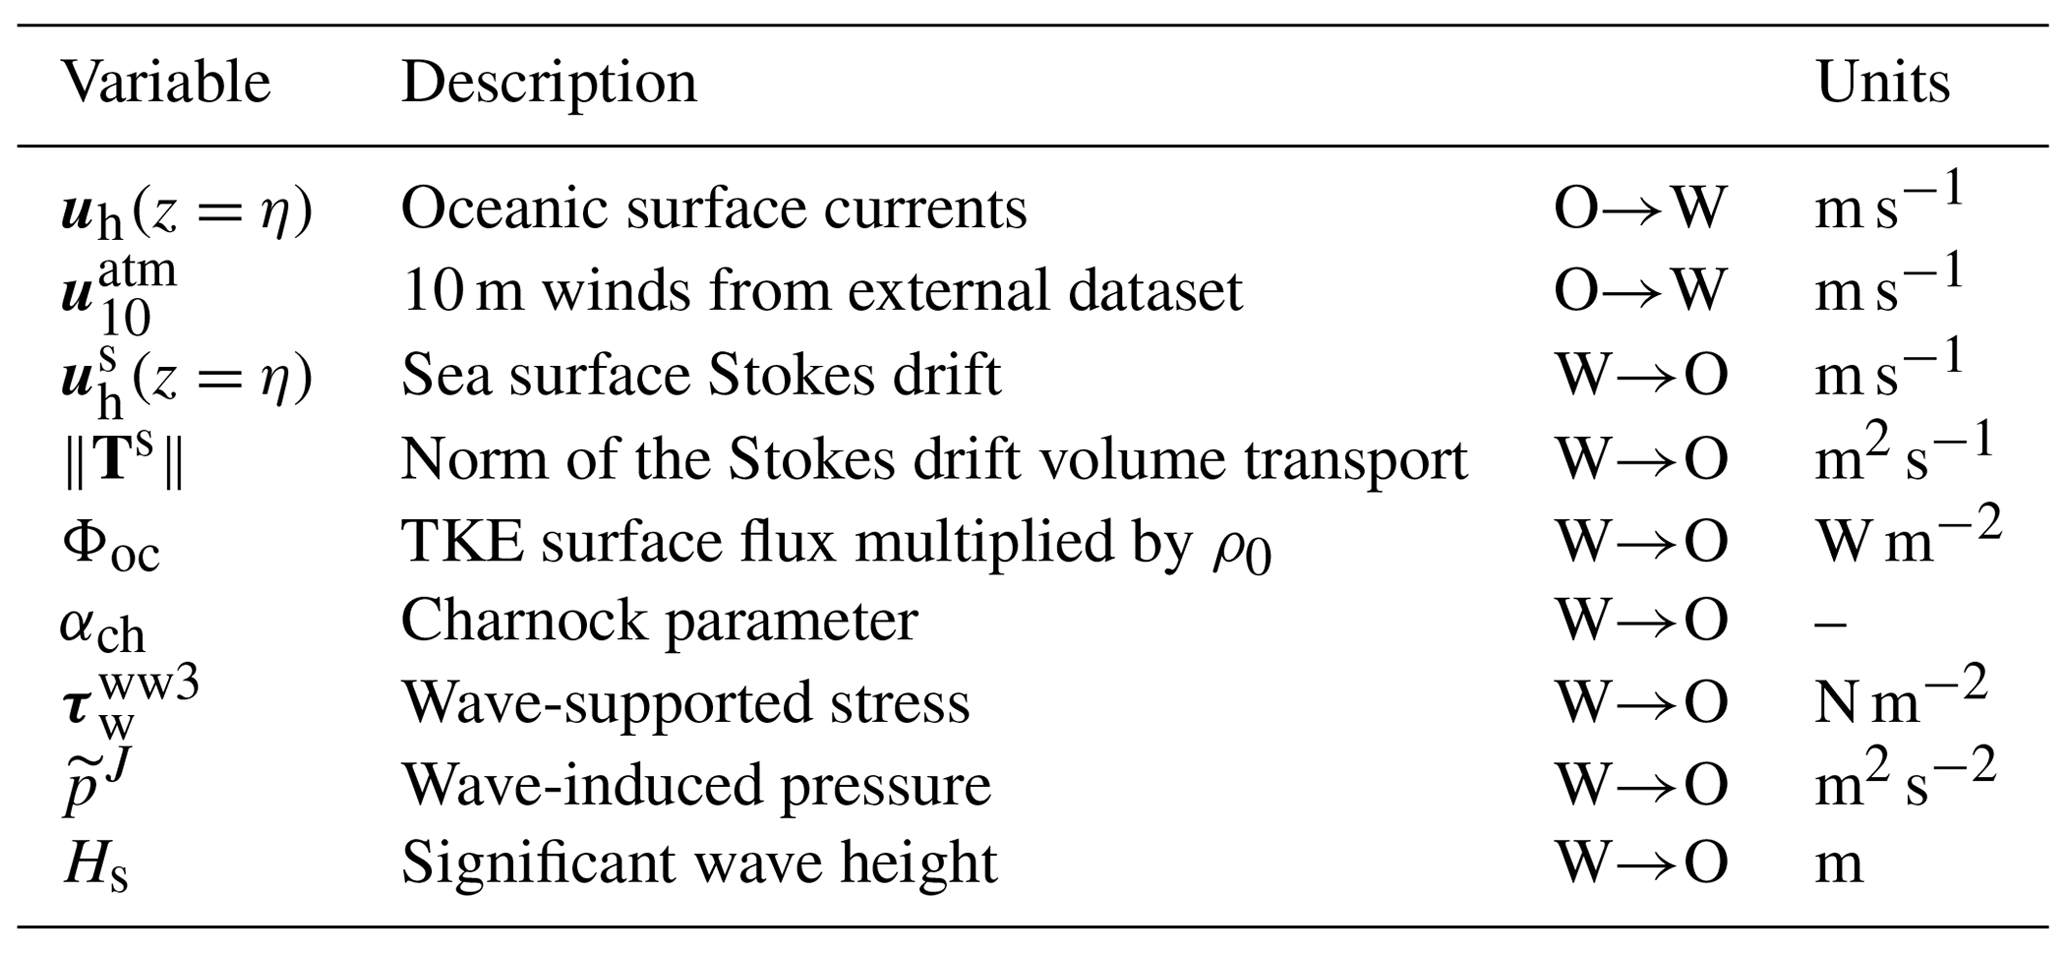
\includegraphics[width=0.5\textwidth]{figures/articles/gmd-13-3067-2020-t01-web.png}
\caption{\label{fig:org82d114e}Tableau tiré de \textcite{couvelard2020development}.}
\end{figure}


\subsection{Analyse dimensionnelle -- \textit{<2023-11-07 Tue>}}
\label{sec:org90c56f3}
\label{org0f74afc}

Avant tout, on n'oublie pas que la contrainte de cisaillement modifiée lorsqu'il y a des vagues est donnée par l'équation \ref{eq:org40e0136}. 
Normalement, lorsqu'on parle d'une contrainte de cisaillement ou d'un stress, les unités sont les même que pour la pression, soit des \(N\cdot m^{-2}\) ou des \(kg\cdot m^{-1}s^{-2}\).
En somme, on les obtient facilement à l'aide de l'équation du frottement visqueux, soit
\begin{align}
   && \boxed{\boldsymbol{\tau}_{A} = \rho_A c_D \abs{\uu_{10}} \uu_{10}\tall }
   && \text{où}\  \tau_A \sim \mathscr{O}\qty(0.1)
   && \text{avec}
   && \tau_A \rightarrow \qty[\frac{kg}{ms^2}],
   && \rho_A \rightarrow \qty[\frac{Kg}{m^3}],
   && \uu_{10} \rightarrow \qty[\frac{m}{s^2}].
\end{align}

Lorsqu'on parle des contrainte de cisaillement du vent et des vagues, on s'attend donc à des \(N m^{-2}\).
Un esprit avisé remarquerait que l'on peut facilement retrouver des unité de stress en multipliant par une densité \(\rho\).
Appellons cette contrainte modifiée \(\tau^*\) pour la différentier,
\begin{align}
   && \boxed{\tau = \rho \cdot \tau^*\tall}
   &&\Longrightarrow
   &&\qty[\qty(\frac{Kg}{m^3})\cdot \qty(\frac{m^2}{s^2})]
   &&\longrightarrow
   &&\qty[ \frac{Kg}{m\pt s^2} ]
   &&\longrightarrow
   &&\qty[\qty(\frac{Kg\cdot m}{s^2})\cdot \qty(\frac{1}{m^2})]
   &&\longrightarrow
   &&\qty[N \cdot m^{-2}]. &&
\end{align}

Mais la question se pose : quelle densité \(\rho\) devons-nous prendre? Celle de l'atmosphère ou celle de l'océan?
Initialement, j'avais pris celle de l'océan (\(\rho_O\)) pour être en accord avec la question des échelles.
Je me souviens qu'on avait eu une discussion là-dessus au milieu de ma maîtrise.

\begin{center}
\begin{tabular}{l|cccc}
\hline
\hline
Quantité à l'étude & \(\tau\)\textsubscript{A} & \(\tau_{fv} = \rho_A\abs{\uu_*}\uu\) & \(\rho_O(\tau_{IN} - \tau_{DS})\) & \(\rho_A(\tau_{IN} - \tau_{IN})\)\\[0pt]
Échelle & \(\sim\) \(\mathscr{O}(0.1)\) & \(\sim\) \(\mathscr{O}(0.1)\) & \(\sim\) \(\mathscr{O}(0.15)\) & \(\sim\) \(\mathscr{O}(0.0002)\)\\[0pt]
\hline
\hline
\end{tabular}
\end{center}

\subsection{Retour sur le cadre théorique -- \textit{<2023-11-07 Tue>}}
\label{sec:orgcbfc5bf}

\subsubsection{Wu et al, 2019 et Breivik, 2015}
\label{sec:org18dc961}

Les articles de \textcite{wu_breivik_2019} et \textcite{breivik_al_2015} représentent explicitement le \emph{wave-supported stress} ( ou le transfert de momentum du vent vers les vagues) par
\begin{equation}
   \boldsymbol{\tau}_{IN} = \rho_O g \int_0^{2\pi} \int_0^{\pt\infty} \qty(\frac{\vb{k}}{\omega} S_{IN} )\pt\mathrm{d}\omega\pt \mathrm{d} \theta,
\end{equation}
Ici, \(\tau\) a des unités de \(N\cdot m^{-2}\).
Donc, les termes reliés au transfert de momentum pour le champ de vagues \(\tau_{IN}\) et \(\tau_{DS}\) sont exprimés par
\begin{equation}
   \boldsymbol{\tau}_{O} = \boldsymbol{\tau}_A - \rho_O g \int_0^{2\pi} \int_0^{\pt\infty} \qty( \frac{\vb{k}}{\omega} \qty(S_{IN} + S_{DS}) )\pt\mathrm{d}\omega\pt \mathrm{d} \theta.
\end{equation}
Ces derniers s'appuient principalement sur \Textcite{bidlot2012present}, \citeauthor*[voir][]{janssen_1989} (\cite*{janssen_1989} et \cite*{janssen_1991}).

\subsubsection{Janssen, 1989}
\label{sec:orgcb3ada1}

Dans un premier temps, \textcite{janssen_1989} décrit le stress du vent avec des unitées de \(N\cdot m^{-2}\).
C'est donc une représentation indépendante de la densité qui est proposée pour le stress du vent.
Dans ce papier, le transfert de momentum du vent proche de l'eau dans la vague elle-même comme une égalité définit par
\begin{equation}
   \boxed{\hspace{0.5cm}
     \underbrace{
       \pdv{}{t} \qty(\rho_A\int_0^{\pt\infty} U_0\pt \mathrm{d}z)\eval{}_{waves}\venti}_{\substack{\text{Momentum transfert from}\\ \text{the airflow to waves}}
       }
     =
     \underbrace{
       -\rho_O \int_0^{\pt\infty} \qty(\omega \pdv{}{t} \phi)\pt \mathrm{d} k \pt\eval{}_{wind}\venti}_{\substack{\text{Momentum transfert from}\\ \text{waves to the wind}}
       } = - \boldsymbol{\tau}_{w} \hspace{0.5cm}
   }
\end{equation}

Concrétement, on peut vraissemblablement représenter ce transfert de momentum à l'aide du comportement du champ de vagues.
Ce qui se traduit par l'utilisation de \(\rho_O\) et \(\rho_A\) dépendemment du référentiel.\bigskip

Hypothétiquement, il se peut que le \(\boldsymbol{\tau}^*\) de Wavewatch III est décrit comme la quantité
\begin{equation}
   \boldsymbol{\tau}^* = \frac{\tau_w}{\rho_A} = \qty(\frac{\rho_O}{\rho_A}) \int_0^{\pt\infty} \qty(\omega \pdv{}{t} \phi) \pt\mathrm{d} k \hspace{0.5cm} \longrightarrow \hspace{0.5cm} \qty[\frac{m^2}{s^2}],
\end{equation}
et c'est ce que l'article de \Textcite{bidlot2012present} semble indiquer à l'aide d'un \emph{air-sea density ratio} (\(\varepsilon\)).


\subsubsection{Janssen, 1991}
\label{sec:org6e8a5dd}

Dans un article subséquent (un article plutôt fondateur), \textcite[voir eq. 7 et 8 de l'article]{janssen_1991}  stipule qu'au repos, on doit respecter l'équation de balance du momentum pour les vagues avec
\begin{equation}
\label{eq:org2b85d2a}
   \boldsymbol{\tau}_w + \boldsymbol{\tau}_{turb} + \boldsymbol{\tau}_{visc}  = \boldsymbol{\tau},
\end{equation}
où \(\boldsymbol{\tau}\) est le stress total définit par \(\boldsymbol{\tau} = \uu_*^2\).
Rapidement, Janssen prend ici une représentation du stress avec des unitées de \(m^{2} s^{-2}\), ce qui nous invite à trouver un \(\rho\) quelque part.
Mathématiquement, le transfert de momentum sur les vagues est exprimé par
\begin{equation}
   \boldsymbol{\tau}_w(z) = - \int_z^{\pt\infty} \mathrm{d}z\pt D_w \pdv[2]{}{z} U_0 \hspace{0.5cm} \longrightarrow \hspace{0.5cm} \qty[\frac{m^2}{s^2}].
\end{equation}
Ici, \(D_z\) est un « coefficient de diffusion des vagues ».
Mentionnons aussi que Janssen se débarasser de \(\omega\) et \(k\) à l'aide d'une condition de résonnance, mais \(D_z\) pourrait s'apparenter à un terme source dans notre nomenclature.
D'ici, il est possible de multiplier toute l'équation \ref{eq:org2b85d2a} par \(\rho_A\) et de se dire que le tour est joué.\bigskip

\nb Dans cet article, Janssen fait apparaitre le concept de \emph{air-sea density ratio}, avec la variable \(\varepsilon\).


\subsubsection{Bidlot, 2012}
\label{sec:org3e8c87e}

\Textcite[voir eq. 6 de l'article]{bidlot2012present} décrit ce tansfert de momentum à l'aide de l'expression
\begin{equation}
   \boldsymbol{\tau}_w = \frac{g}{\varepsilon} \int \mathrm{d}\omega\pt \mathrm{d}\theta\pt S_{IN} \vb{k} = \qty(\frac{\rho_O}{\rho_A}) \int \mathrm{d}\omega\pt \mathrm{d}\theta\pt g\pt S_{IN} \vb{k}.
\end{equation}
Avec \(S_{IN} = \gamma N\).
Et c'est ici qu'on voit finalement apparaître le \emph{air-sea density ratio} (\(\varepsilon\)).
Notamment, \(\tau_w\) est ici une quantité donnée en \(m^2\pt s^{-2}\) et c'est d'ailleurs la formulation qui est utilisée dans ECWAM.
Donc, est-ce que le \(\tau_{IN}\) offert par Wavewatch III est ouvertement divisé par \(\rho_A\) avant d'être transmis en \emph{output}?
\emph{The plot thickens\ldots{}}

\subsubsection{Que dit le code de Wavewatch III? -- \textit{<2023-11-08 Wed>}}
\label{sec:org1120859}

Après un peu de recherche, le code ne peut pas être plus clair (voir figure \ref{fig:org241ebba}). 

\begin{figure}[htbp]
\centering
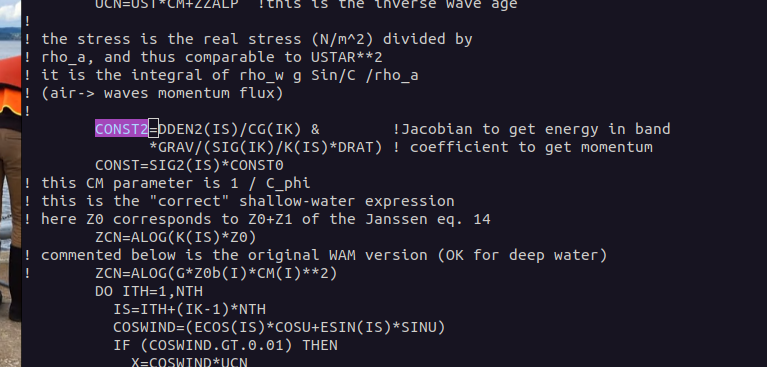
\includegraphics[width=.9\linewidth]{figures/articles/Screenshot from 2023-11-08 15-59-22.png}
\caption{\label{fig:org241ebba}«Screenshot» du code de Wavewatch où ils sont assez explicites sur la nature de \(\tau_{IN}\).}
\end{figure}


\nb \textbf{L'expérience de pensée qu'il faut faire} : On se fout de l'eau ou plutôt du matériau de la vagues.
La vague pourrait être en roche ou en lave, le transfert de momentum de l'air sur la surface ondulée reste exactement le même.
Ensuite, le momentum va faire réagir la surface ondulée ou le mur dépendement de la densité du matériau.
Mais le momentum qu'on retire au vent ne dépend tout simplement pas de la densité de l'eau. \bigskip



\section{Rencontre -- \textit{<2023-11-09 Thu>}}
\label{sec:orgfaefaa2}

On veut absolument comparer l'effet des vagues sur l'énergie, en tout cas.

Les effets de la \emph{roughness lenght}.

Liste d'épicerie :
\begin{itemize}
\item Vent constant versus hautes fréquences.
\item Couplé et non-couplé.
\end{itemize}

Faut juste le faire.

Au début : \emph{thickness} va à zéro. Quick fix. 

\printbibliography
\end{document}